\documentclass[10pt,a4paper,twocolumn]{article}
\RequirePackage[italian]{babel}
\usepackage[utf8]{inputenc}
\usepackage{amsmath}
\usepackage{amsfonts}
\usepackage{amssymb}
\usepackage{graphicx}

\author{M. Faretra, G. Marini, A. Martinelli}
\title{\textbf{Raccolta accurata di fatti da testo in linguaggio naturale di Wikipedia}}
\begin{document}
	
\maketitle
		
\section*{RIASSUNTO}
		
Molti approcci sono stati tentati nell'ultimo periodo per estrarre informazione da Wikipedia sotto forma di fatti (entità, relazione, entità) per il popolamento di Knowledge Graphs, in particolare sfruttando le informazione contenute nelle sue \textit{infoboxes}. Tuttavia queste strutture dati riportano solo una piccola parte delle informazioni contenute negli articoli. Infatti nel testo libero si concentra la maggior parte delle relazioni estraibili, tuttavia la rilevazione di esse risulta più problematica trovandosi all'interno di linguaggio naturale e non ben evidenziato come accade nelle infoboxes. In questo lavoro si cerca di quantificare il numero di nuovi fatti estratti da questi articoli con il supporto di un KG già popolato per aumentarne la conoscenza. In particolare, la nostra valutazione è stata effettuata utilizzando DBpedia, un KG gratuito, che ci ha portato a... (discuss to be implemented, un paio di numeri sui risultati che poi verranno discussi meglio)

\section{INTRODUZIONE} 

L'incremento dei Knowledge Graph in questi ultimi tempi è stata di particolare interesse scientifico e ha evidenziato la limitatezza e la mancanza di informazioni in essi presente, dovuta in alcuni casi a entità inserite automaticamente senza particolari relazioni, in altri alla limitata conoscenza reperibile dagli infoboxes.

Il progetto DBpedia estrae informazioni da più di 125 edizioni in linguaggi differenti di Wikipedia. La più grande base di conoscenza è estratta dalla versione inglese e consiste in più di 580 milioni di fatti che descrivono 38 milioni di cose. DBpedia estrae informazione dal testo di  Wikipedia da 28 edizioni in linguaggi differenti in una singola ontologia condivisa consistente di circa 685 classi e 2795 proprietà. 

La conoscenza estraibile dal testo libero potrebbe essere decisamente più consistente e aumentare di molto il Knowledge Graph. L'approccio utilizzato va a scalare sfruttando i fatti contenuti nel KG stesso, è quindi dipendente anche da essi, ed in particolare dalla loro qualità: le triple sono etichettate come fidate e non fidate e con esse abbiamo effettuato misurazioni differenti, considerando le relazioni candidate estratte dalle triple appartenenti all'una o all'altra categoria.

L'utilizzo di Wikipedia è ampiamente diffuso tra i vari KG esistenti data la grande affidabilità che ormai garantisce, tuttavia le infoboxes fino a pochi anni fa erano ancora molto poco diffuse e solo nell'ultimo decennio esse si trovano in più della metà degli articoli. Nonostante la presenza di dataset relativi al testo libero, per il nostro lavoro abbiamo sfruttato per l'estrazione quello di DBpedia costruito a partire da questa struttura dati.

Se invece si va a considerare la conoscenza presente nel testo libero, si può immaginare che da esso (ovviamente presente in ogni articolo) si possa estrarre informazione non presente nel KG poiché esso riporta una serie di relazioni che probabilmente non sono presenti nell'infobox, ad esempio riguardanti entità che non sono il soggetto dell'articolo.

Il nostro approccio al problema considera pattern del tipo 
"[entità] frase [entità]", ad esempio: "Francesco Totti was born in Rome" mette in relazione le due entità "Francesco Totti" e "Rome" utilizzando la frase "was born in" che descrive un'istanza della relazione "birthPlace".
In questo articolo descriviamo l'approccio di estrazione di conoscenza da testo libero di Wikipedia, e i risultati in termini di aumento dei fatti presenti in DBpedia, che usiamo per verificare l'effettiva validità della frase per esprimere una determinata relazione.
Per l'estrazione abbiamo generato dal dump in input triple candidate a rappresentare informazione valida, verificando se la frase della tripla sia o meno relazionale e confrontandole con il KG per estrarre nuovi fatti.
(discuss sommaria spiegazione del processo e qualche numero di risultati)
Il resto dell'articolo è organizzato in vari capitoli: nel Capitolo 2 vengono analizzate in maggior dettaglio le risorse utilizzate; nel Capitolo 3 si presenta il nostro approccio; nel Capitolo 4 vengono mostrati i nostri risultati; nel Capitolo 5 si trovano cenni a lavori correlati e su cui ci siamo basati (discuss se vogliamo scriverci qualche cagata su Lector da cui siamo partiti); infine, nel Capitolo 6 vengono presentate le conclusioni sul lavoro effettuato.

\section{RISORSE}
\subsection*{\textit{Wikipedia.}}

Wikipedia è un'enciclopedia online libera e collaborativa, che attualmente comprende circa 5.3 milioni di articoli nella sua versione inglese. Questa modalità di collaborazione garantisce una grande qualità e affidabilità sulle informazione ed anche una certa omogeneità nell'esprimere determinati concetti che va a facilitare l'estrazione di fatti.
 
Ogni articolo in Wikipedia fa riferimento ad una entità principale, che può rappresentare una persona, un luogo, un oggetto, un fatto, ecc..., identificata da un identificatore. Nel testo le informazioni sono codificate in linguaggio naturale, inoltre le entità secondarie eventualmente presenti in un determinato articolo sono rappresentate usando dei \textit{wikilinks}, una sintassi specifica di Wikipedia per evidenziare un particolare concetto e offrire un link all'articolo che lo descrive per avere un quadro più generale sulla questione.

Nel nostro particolare caso le frasi di Wikipedia su cui lavorare ci sono state fornite dal docente poichè il progetto è stato svolto in ambito universitario, nella forma di sentenze con le entità già etichettate in una particolare modalità:
\bigbreak
\textit{[[Barack\_Obama$|$m.02mjmr]] met [[Donald\_Trump$|$m.0cqt90]] after the elections.}
\bigbreak
Come si può vedere le entità sono ben identificate e quindi di facile estrazione, e possiedono anche un id che rappresenta l'entità all'interno di Freebase, quindi non rilevante per questa trattazione.

\subsection*{\textit{DBpedia.}}

DBpedia è frutto di un lavoro di collaborazione da parte di una moltitudine di utenti per estrarre informazioni strutturate da Wikipedia e renderle disponibili sul Web.

Ogni "cosa" in DBpedia è identificata da un URI del tipo:
\bigbreak
\textbf{http://dbpedia.org/resource/Name}
\bigbreak
dove "Name" è preso dall'URL del relativo articolo di Wikipedia, che ha la forma:
\bigbreak
\textbf{http://en.wikipedia.org/wiki/Name}.
\bigbreak
In questo modo ogni risorsa è legata direttamente ad un articolo di Wikipedia. I dati sono suddivisi in dataset diversi ed in particolare quelli che abbiamo preso in considerazione per il progetto sono due (discuss sono davvero solo 2?):
\begin{itemize}
\item quello relativo ai tipi delle entità, ovvero una serie di coppie "URL entità - URL tipo", che associa ad esempio all'entità "Barack Obama" il tipo "Persona";
\item un dataset relativo agli schema e ai collegamenti tra entità e relazioni utilizzati da DBpedia che analizzeremo in seguito
\end{itemize}

\section{APPROCCIO}

Il dataset iniziale di frasi, come detto precedentemente, ci è stato fornito con le entità etichettate. Inizialmente abbiamo provato ad applicare un approccio euristico per il riconoscimento di frasi di tipo lista, basato su un lavoro precedentemente svolto da alcuni colleghi, che si è rivelato non scalabile. Si è quindi preferito perdere parte dell'informazione in esse presente favorendo la velocità, data la grande mole di dati.
Il processamento si svolge in diversi passaggi:
\begin{enumerate}
\item Verifica della relazionalità della frase in questione;
\item Etichettatura delle triple "presenti" e "non presenti";
\item Scoring delle frasi;
\item Estrazione di informazione.
\end{enumerate}

\subsection{Verifica delle frasi}
Il dump iniziale delle frasi ci è stato fornito dal professore con le entità delimitate da parentesi quadre e arricchite con l'id relativo su \textit{Freebase}, superfluo per questo lavoro. Il dato all'interno di esse ci fornisce il \textit{wikid} che ci è stato utile per reperire l'entità anche su DBpedia, che usa proprio questi identificatori per salvarle, poiché basato proprio su Wikipedia. In alcuni casi questi identificatori fanno riferimento ad un \textit{redirect} che punta all'effettivo wikid che abbiamo reperito tramite una mappatura offerta da un altro file di input fornito dal docente.

Abbiamo quindi suddiviso le frasi iniziali in una lista di triple comprendenti tutte le coppie di entità e il testo compreso tra esse, perdendo parte dell'informazione presente ad esempio in frasi di tipo lista nelle quali il soggetto andrebbe collegato con le varie entità in relazione con esso utilizzando il pezzo di frase che lo collega con la prima entità. 
\begin{figure}[h]
	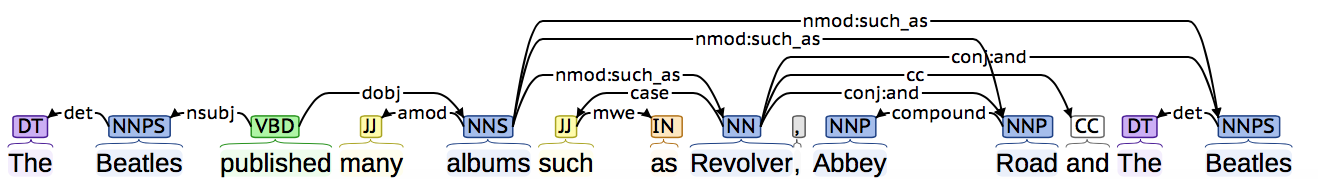
\includegraphics[width=7.8cm, height=1.2cm]{stanford}
	\caption{Esempio di una frase di tipo lista}
\end{figure}
 (discuss eventuale immagine di stanford?).

Le frasi tra le entità sono state quindi passate ad un filtro per trovare quelle di tipo relazionale. Questa operazione snellisce di molto il dataset iniziale eliminando la maggior parte degli spezzoni di testo tra entità poiché il filtro è molto restrittivo, garantendo dall'altra parte un output di frasi che quasi sicuramente esprime una relazione tra due entità.

\subsection{Etichettatura}
A questo punto, abbiamo considerato le entità di ogni tripla per verificarne l'effettiva presenza all'interno di DBpedia.

Le triple "etichettate" rappresentano fatti già presenti nel KG e sono utili per ricavare una mappatura tra le frasi che legano le entità e le relazioni ad esse accomunabili.

Quelle non etichettate sono invece candidate a rappresentare quella parte di conoscenza che il nostro lavoro va a reperire in più, ampliando l'informazione della base di conoscenza.

Le frasi hanno subito uno \textit{stemming} per pulire le frasi e ricondurre quelle più particolari a forme più generali in modo da non perdere informazione.

\subsection{Scoring}

Ogni frase di quelle non etichettate è associata ad una o più relazioni provenienti da DBpedia, ma ovviamente queste corrispondenze potrebbero essere non veritiere. Abbiamo quindi assegnato ad ogni frase un punteggio per l'appartenenza o meno ad una relazione considerando il numero di volte che esse sono associate. In questo modo abbiamo cercato di penalizzare frasi che esprimono concetti molto generici poiché non danno molta fiducia sulla correttezza dell'associazione.

Il punteggio viene assegnato tenendo conto del numero di volte che la frase è collegata alla determinata relazione ( $c(p,r_i)$ ), al conteggio totale delle sue occorrenze in tutte le relazioni ( $\sum_{j \in R} c(p,r_j)$ ) e al numero di relazioni a cui è associata ( $c(R|p)$ ) secondo la seguente formula: (suddividere la formula con la parte centrale raccolta nella probabilità)
\[score(p,r_i)=c(p,r_i)\cdot\frac{c(p,r_i)}{\sum_{j \in R}c(p,r_j)}\cdot \frac{1}{c(R|p)} \]
In questo modo una frase ottiene un punteggio maggiore quanto più compare associata alla relazione in questione rispetto al numero totale di occorrenze, penalizzando le frasi in base al numero di relazioni a cui sono associate, poiché si tratta di forme con molta generalità e utilizzate per esprimere un grande insieme di relazioni diverse. 

\subsection{Estrazione dell'informazione}

Nella parte finale prendiamo le 20 frasi (o tutte se ce ne sono meno) con punteggio più alto per ogni relazione e le utilizziamo con le entità che mettono in relazione nelle triple per estrarre fatti. La frase per essere valida deve essere presente per la relazione in questione su DBpedia, ed inoltre, ogni tripla, per essere considerata valida, deve rispettare i tipi che la relazione collega su DBpedia. Ad esempio, la frase "\textit{was born in}" è valida per la relazione \textit{birthPlace} se la prima entità è del tipo "Person" e la seconda del tipo "Location".

\section{VALUTAZIONE}

\end{document}